\documentclass[a4paper,11pt]{article}
\usepackage{a4wide}
\usepackage{fullpage}
\usepackage[utf8x]{inputenc}

\usepackage[light,math]{anttor}
\usepackage[T1]{fontenc}

%\usepackage[slovene]{babel}
%\selectlanguage{slovene}
\usepackage[toc,page]{appendix}
\usepackage[pdftex]{graphicx} 

\usepackage{lmodern}
\usepackage{amsmath}
\usepackage{amssymb}
\usepackage{amsthm}
\usepackage{amsfonts}
\usepackage{mathtools}
\usepackage{enumitem}
\usepackage{amsfonts}
\usepackage{setspace}
\usepackage{color}
\definecolor{light-gray}{gray}{0.95}
\usepackage{listings} 
\usepackage{hyperref}
\usepackage[english, croatian, slovene]{babel}

\renewcommand{\baselinestretch}{1.2} 
\renewcommand{\appendixpagename}{Priloge}


\title{Teorija grafov \\
\textbf{Domača naloga} }
\author{Sara Bizjak  |  IŠRM  |  27202020}
\date{April 2021}

%%%%%%%%%%%%%%%%%%%%%%%%%%%%%%%%%%%%%%%%%%%%%%%%%%%%%%%%%%%%%%%%%%%%%%%%%%%%%%%%%%%%%%%%%%%%%%%%%%%%%%%%%%%%%%%%%%%%%%%%%%%%%%%%%

\begin{document}

\maketitle

%%%%%%%%%%%%%%%%%%%%%%%%%%%%%%%%%%%%%%%%%%%%%%%%%%%%%%%%%%%%%%%%%%%%%%%%%%%%%%%%%%%%%%

\noindent
Naloge sem reševala samostojno.
Pri reševanju sem si pomagala z zapiski predavanj in vaj ter z gradivom, ki sem ga našla na internetu.

\section*{1. naloga}
Za vsak $k \geq 2$ najdi $k$-regularen graf, ki nima popolnega prirejanja. Odgovor utemelji.
\\

\noindent
Problem razdelimo na dva primera in opazujemo grafe posebej za sode in posebej za lihe $k$.
\\

\noindent
\begin{itemize}
\item \textit{$k$ je sod}. 
    \begin{itemize}[label={}]
        \item Iskani $k$-regularen graf za sode $k$ je polni graf na $k + 1$ vozliščih ($K_{k + 1}$). To je res, saj bi za popolno prirejanje število vozlišč v polnem grafu moralo biti sodo, $k + 1$ pa je liho število, torej popolnega prirejanja ni.
                Poglejmo si skici za prva dva takšna primera, torej za $k = 2$ in $k = 4$.

                        \begin{figure}[ht!]
                            \centering
                            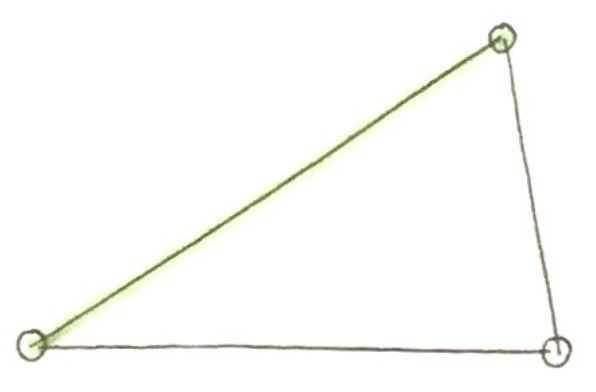
\includegraphics[width=50mm]{Slike/k_sod_1.png}
                            \caption{Graf za $k = 2 \rightarrow K_3$.}
                        \end{figure}
                        \noindent
                        Popolnega prirejanja očitno ni, saj vozlišča nasproti prve povezave, ki jo dodamo v prirejanje (označeno z zeleno barvo), ne moremo zasiši z nobeno povezavo. Če bi ga, potem prirejanje ne bi bilo popolno.
                                
                        \newpage
                        \begin{figure}[ht!]
                            \centering
                            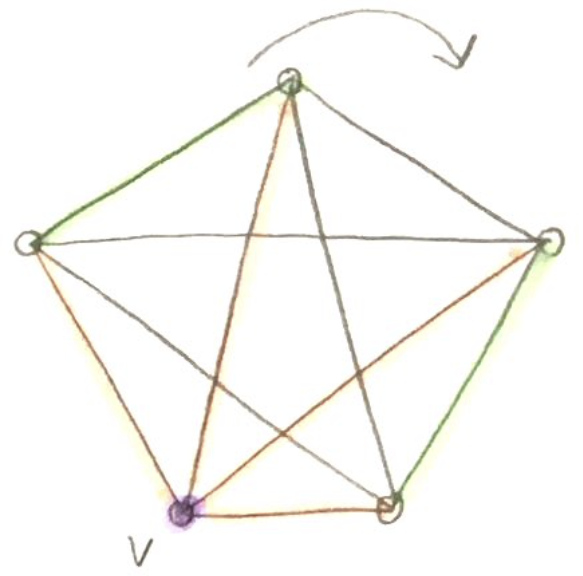
\includegraphics[width=50mm]{Slike/k_sod_2.png}
                            \caption{Graf za $k = 4 \rightarrow K_5$.}
                        \end{figure}
                        \noindent
                        BŠS lahko začnemo dodajati zunanje povezave v izbrani zmeri (označeno z zeleno barvo in puščico). Vozlišča v (označenega z vijolično barvo) tedaj ne moremo zasičiti z nobeno povezavo, saj če bi dodali katerokoli oranžno povezavo v prirejanje, ne bi bilo popolno.
    
    \end{itemize}

\item \textit{$k$ je lih.}
    \begin{itemize}[label={}]
        \item Zamislimo si naslednji graf. Graf začnemo risati v enem (začetnem) vozlišču in ga povežemo s $k$ naslednjimi vozlišči. Vsako izmed teh $k$ vozlišč povežemo s $k - 1$ novimi in potem še teh $k - 1$ povežemo z naslednjimi $k - 1$ tako, 
        
                da bodo vsa vozlišča na eni strani povezana z vsemi vozlišči na drugi (tako, da na tem delu nastane $K_{k-1, k-1}$). 
                Zadnjih dodanih vozlišč je sodo mnogo ($k - 1$), povežemo še dve po dve skupaj.
                \\
                Vsako vozlišče v tako konstruiranem grafu ima natanko $k$ sosedov, torej je graf res $k$-regularen.
                \\
                Za dokaz o neobstoju $1$-faktorja (kar je ekvivalentno temu, da graf nima popolnega prirejanja) uporabimo Tuttov izrek. Za množico $S$ izberemo začetno vozlišče. Če iz grafa $G$ odstranimo začetno vozlišče ($G - S$), dobimo natanko $k$ lihih komponent, vsako s po $1 + (k - 1) + (k - 1)$ vozlišči. Ker je $\sigma (G - S) = k > |S| = 1$, tak graf po Tuttovem izreku ne premore $1$-faktorja, torej nima popolnega prirejanja.
                \\
                Za lažjo predstavo konstrukcije grafa si poglejmo skico za najmanjši tak primer, torej $k = 3$.
                \\
                Pri grafu za $k = 3$ velja: Naj bo oranžno (začnetno) vozlišče označeno z $u$ in naj bo $S = \{ u\}$ v Tuttovem izreku. 
                Tedaj $\sigma(G - S) = 3 > |S| = 1$, kar pomeni, da graf res ne premore popolnega prirejanja.
                \begin{figure}[ht!]
                    \centering
                    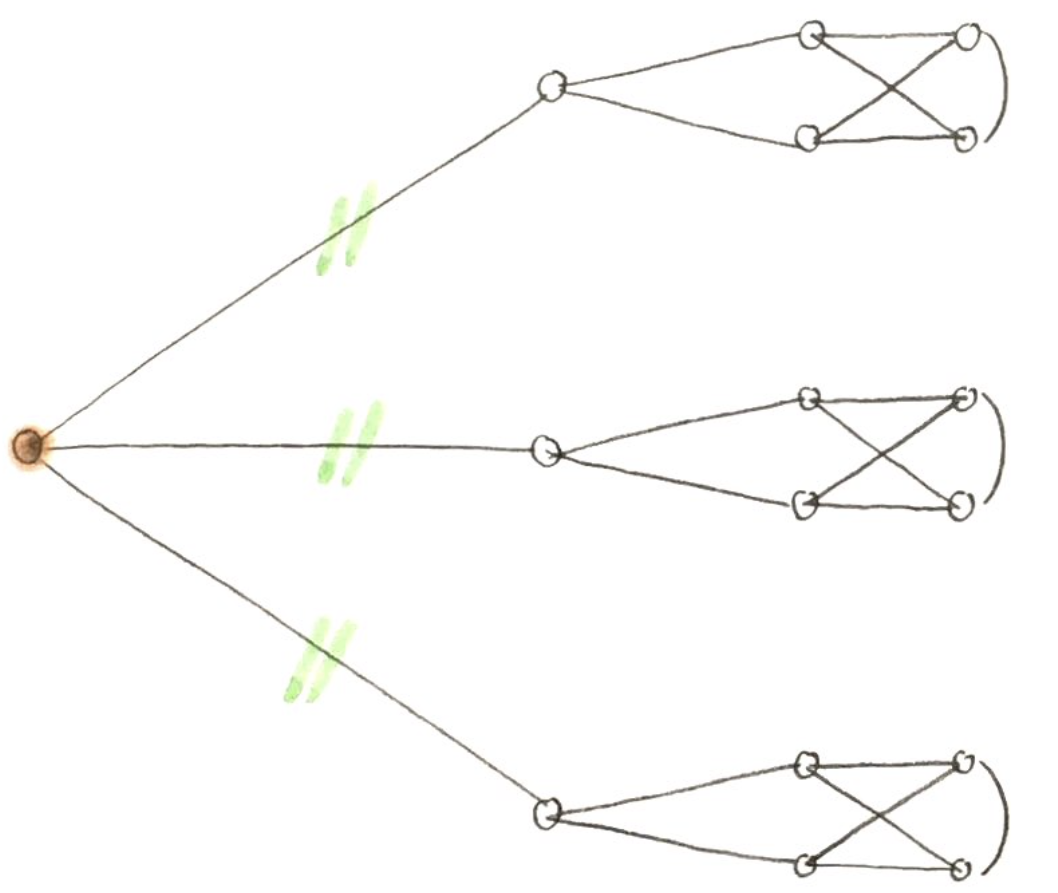
\includegraphics[width=80mm]{Slike/k_lih.png}
                    \caption{Graf za $k = 3$.}
                \end{figure}
    \end{itemize}
\end{itemize}
%%%%%%%%%%%%%%%%%%%%%%%%%%%%%%%%%%%%%%%%%%%%%%%%%%%%%%%%%%%%%%%%%%%%%%%%%%%%%%%%%%%%%%%%%%%%%%%%

\newpage
\section*{2. naloga}

%%%%%%%%%%%%%%%%%%%%%%%%%%%%%%%%%%%%%%%
\textbf{A del:}
Naj bo $H$ graf brez izoliranih vozlišč, v katerem je vsaka povezava incidenčna z vozliščem stopnje $1$. Opiši povezane komponente grafa $H$. Dokaži, da je $\alpha^{'}(H) \geq \frac{|V(H)|}{\Delta (H) + 1}$.
\\
\\
Če je vsaka povezava incidenčna z vozliščem stopnje $1$, potem vsako tako vozlišče predstavlja list in komponente grafa so 'zvezde' (prikazano na sliki \ref{zvezda}).
\begin{figure}[ht!]
    \centering
    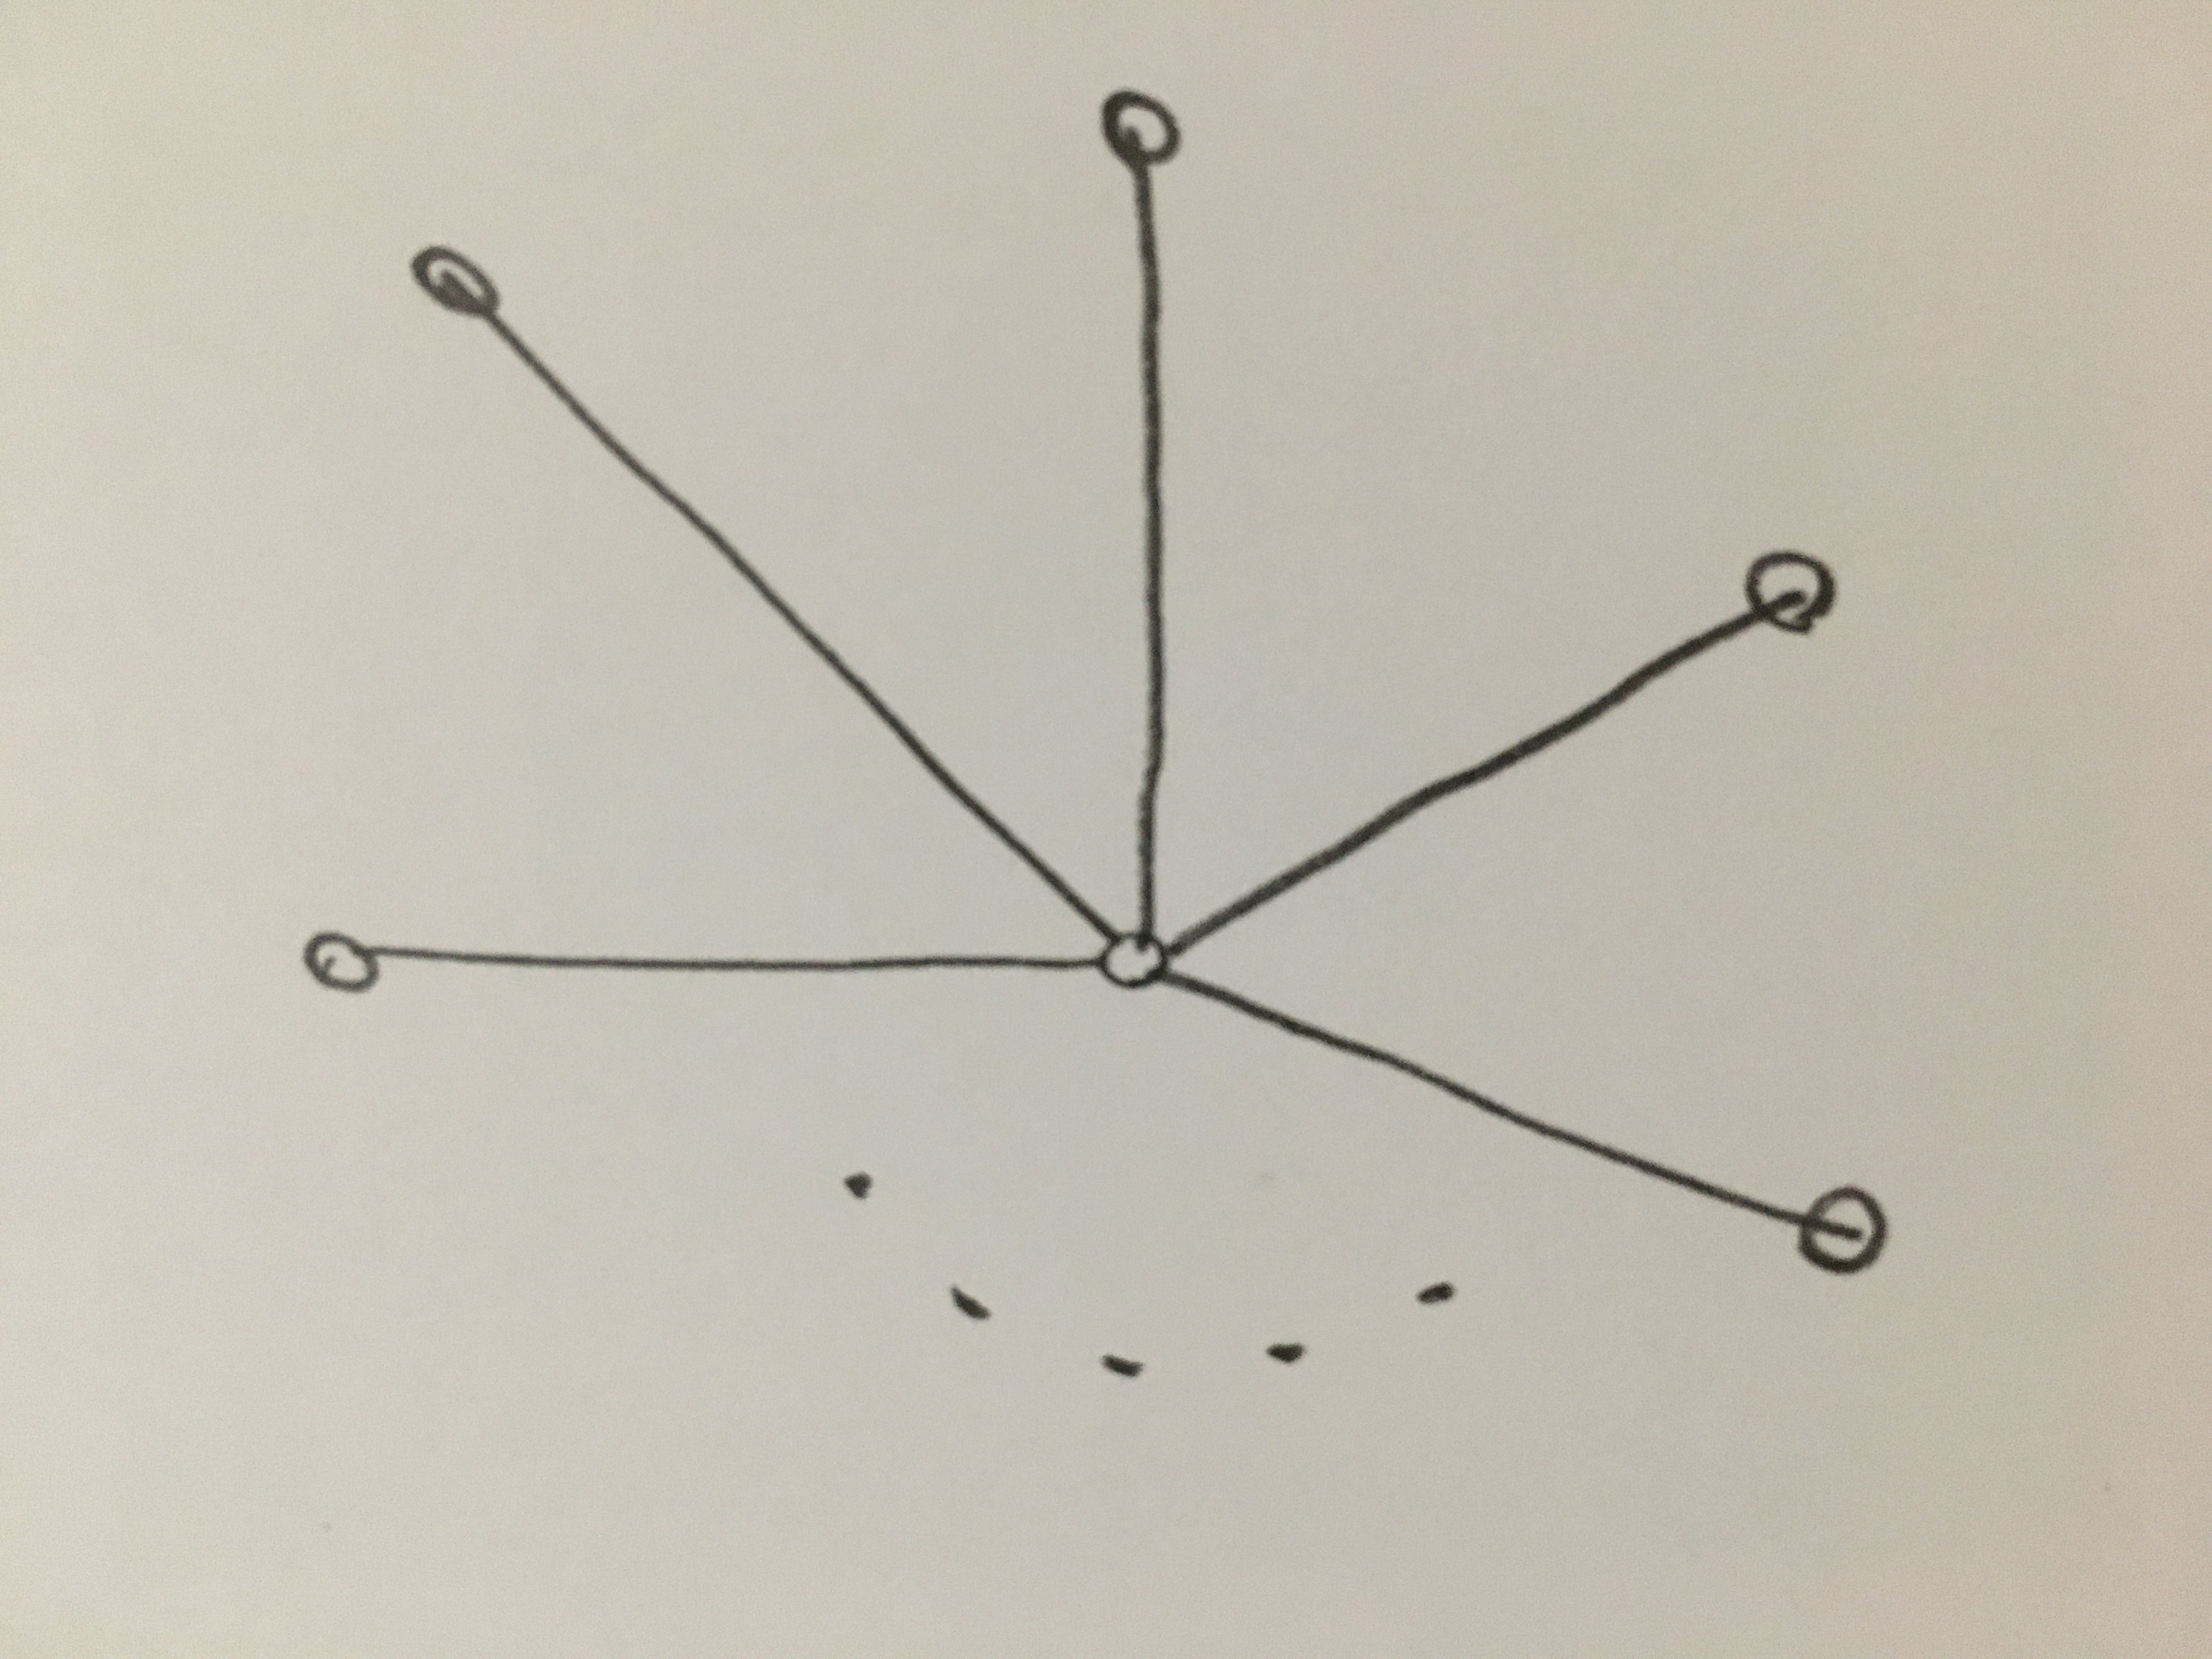
\includegraphics[width=80mm]{Slike/zvezda.JPG}
    \caption{Komponenta grafa $H$.}\label{zvezda}
\end{figure}

\noindent
Najprej opazujmo graf $H$ z eno samo komponento.
Največje prirejanje za $H$ je očitno velikosti $1$. 
Denimo, da ima graf $n + 1$ vozlišč. Sredinsko vozlišče ima tako stopnjo enako $n$, kar je tudi maksimalna stopnja grafa, torej $\Delta(H) = n$, torej očitno velja $1 = \alpha^{'}(H) \geq \frac{|V(H)|}{\Delta (H) + 1} = \frac{n + 1}{n + 1} = 1$. 
\\
Naj ima sedaj graf več komponent. V tem primeru je razmislek podoben. Največje prirejanje bo tako enako številu komponent, denimo, da jih je $h$ mnogo.
Maksimalna stopnja grafa bo enaka stopnji sredinskega vozlišča v največji komponenti, recimo, da je, kot prej, enaka $n$. 
Ker je $n$ maksimalna stopnja vozlišča, je potem največja komponenta velika $n + 1$. Ker nobena komponenta ni večja od $n + 1$, je zgornja meja za vozlišča vseh komponent skupaj enaka $h \cdot (n + 1)$. Iz tega sledi
$$
h = \alpha^{'}(H) \geq \frac{h \cdot (n + 1)}{n + 1} = h
$$
Če so torej vse komponente enako velike, velja enakost, sicer imamo strogi neenačaj, saj bo izraz v števcu strogo manjši od $h \cdot (n + 1)$.
\\

%%%%%%%%%%%%%%%%%%%%%%%%%%%%%%%%%%%%%%%



\noindent
\textbf{B del:}
Dokaži, da za vsak graf $G$ brez izoliranih vozlišč velja $\alpha^{'}(H) \geq \frac{|V(H)|}{\Delta (H) + 1}$.
\\
\\
Ideja je indukcija po številu povezav grafa $G$.
\\
\textit{Baza indukcije.} Graf $G$ brez izoliranih vozlišč z eno povezavo (to sta dve vozlišči povezani med sabo) in pogoj velja.
\\
\textit{Indukcijska predpostavka.} Denimo, da pogoj velja za vse grafe, ki imajo največ $k$ povezav.
\\
\textit{Indukcijski korak.} Pogoj bi sedaj radi dokazali za graf $G$, ki ima $k + 1$ povezav. V tem grafu izbereno vozlišče $v = \Delta(G)$ in enega od njegovih robov, označimo z $e$, ki ga iz grafa odstranimo.
Obravnavamo tri primere:
\begin{itemize}
    \item Če odstranimo $e$, izoliramo obe robni vozlišči povezave. V tem primeru je $deg(v) = 1$, torej je $\Delta(G) = 1$, saj smo za $v$ izbrali tako vozlišče z maksimalno stopnjo.
        Če odstranimo še obe ti dve vozlišči, ki sta po odstranitvi povezave $e$ izolirani, dobimo graf s $G^{'}$ s $k$ povezavami brez izoliranih vozlišč, kar zadošča naši indukcijski predpostavki ($\alpha^{'} (G^{'}) \geq \frac{k}{2}$).
        Očitno potem za $G$ velja $\alpha^{'} (G) \geq \frac{k + 1}{2}$, saj sta obe robni vozlišči povezave $e$ stopnje $1$, torej tudi to povezavo lahko dodamo v prirejanje in bo množica še vedno neodvisna.
    \item Če odstranimo $e$, izoliramo eno od obeh robnih vozlišč. Izolirano vozlišče v tem primeru gotovo ni $v$, saj sicer ne bi bilo maksimalne stopnje. Podobno kot prej sedaj iz grafa $G - e$ odstranimo še izolirano vozlišče. Tako dobimo graf, ki zadošča indukcijski predpostavki $\alpha^{'} (G^{'}) \geq \frac{k}{\Delta(G^{'}) + 1}$.
        Očitno je, da je $\Delta(G) = \Delta(G^{'}) + 1$, saj ima vozlišče $v$, ki je maksimalno, eno povezavo več v $G$ kot v $G^{'}$ ($e$). Iz tega sledi, da $\alpha^{'} (G) \geq \frac{k + 1}{\Delta(G^{'}) + 2} = \frac{k + 1}{\Delta(G) + 1}$, saj je največje prirejanje $G$ lahko kvečjemu za 1 večje od največjega prirejanja za $G^{'}$.
    \item Če odstranimo $e$, ne izoliramo nobenega vozlišča. Torej lahko induktivno predpostavko direktno apliciramo in pogoj velja.
\end{itemize}
%%%%%%%%%%%%%%%%%%%%%%%%%%%%%%%%%%%%%%%%%%%%%%%%%%%%%%%%%%%%%%%%%%%%%%%%%%%%%%%%%%%%%%%%%%%%%%%%
\newpage
\section*{3. naloga}
Naj bo $G$ $k$-povezan graf na vsaj $2k$ vozliščih. Dokaži, da v grafu $G$ obstaja cikel dolžine vsaj $2k$.
\\
\\
Najprej premislimo, da v $G$ obstaja cikel.
Kerj velja
\begin{align}\label{1}
    \delta (G) \geq \kappa (G) \geq k \geq 2
\end{align}
graf ni drevo, torej im cikel.
\\
Označimo sedaj s $C$ najdaljši cikel v $G$. Po \ref{1} vemo, da $|C| \geq k + 1$. Dokazali bi radi, da $|C| \geq 2k$. 
\\
Pokažimo to s protislovjem. Denimo, da $|C| < 2k$. 
\\
Označimo z $v$ vozlišče, ki ni v $C$, torej $v \in G \backslash C$, kot je prikazano na sliki \ref{graf}.
\begin{figure}[ht!]
    \centering
    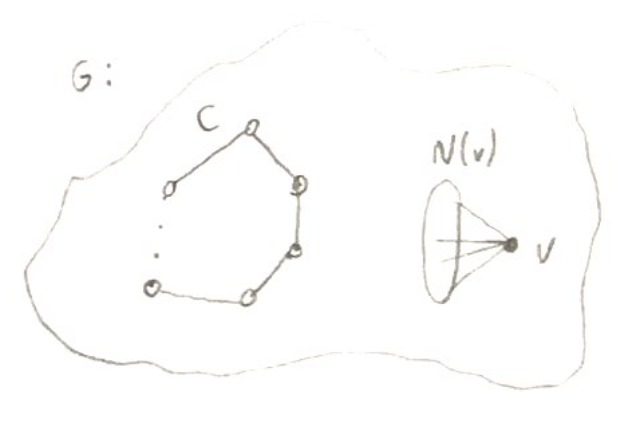
\includegraphics[width=80mm]{Slike/3_graf.png}
    \caption{Graf $G$.}\label{graf}
\end{figure}
Po \ref{1} velja, da je $|N(v)| \geq k$. Vemo še, da nobena množica manjša od $k$ ne more loćiti $N(v)$ od $V(C)$, saj je $G$ $k$-povezan.
Z drugimi besedami: vemo, da je moč najmanjše prerezne množice bsaj $k$. Iz tega po Mengerju sledi, da je med $N(v)$ in $V(C)$ vsaj $k$ disjunktnih poti.
\\
Naj bosta sedaj $v_1, v_2 \in N(v)$ in $c_1, c_2 \in C$. Tedaj obstajata različni poti $a_1c_1$ in $a_2c_2$, ki ju označimo $P_1$ in $P_2$ po vrsti. Pot med $c_1$ in $c_2$ označimo s $P$.
\\
Ločimo dve možnosti:
\begin{itemize}
    \item $v \notin P_1, v \notin P_2$. Prikazano na sliki \ref{pot1}.
        \\
        Naj bo $C^{'} = v P_1 P P_2$ v nov cikel, ki je očitno daljši, če za pot med $c_1$ in $c_2$ vzamemo pot okoli po ciklu $C$ (kot pobarvano na sliki).
        \begin{figure}[ht!]
            \centering
            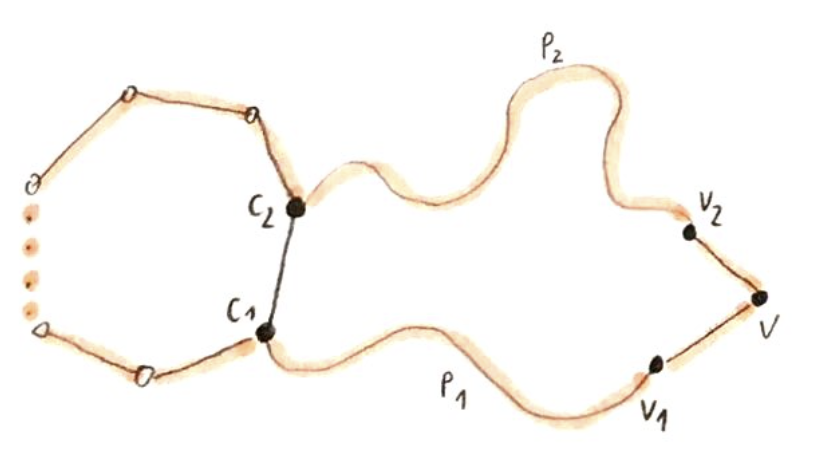
\includegraphics[width=80mm]{Slike/3_1.png}
            \caption{Primer, ko $v \notin P_1, v \notin P_2$.}\label{pot1}
        \end{figure}
        Ta cikel je res vsaj za $1$ daljši, saj $|(C - c_1c_2)| + |P_1| + v_1v - vv_2 + |P_2| \geq |C| - 1 + 2 = |C| + 1$.

    \item $v \in P_1$ (BŠS). Prikazano na sliki \ref{pot2}.
        \\
        Označimo s $P_1^{'}$ pot od $c_1$ do $v$ vzdolž $P_1$. Tedaj je $C^{'} = v P_1^{'} P P_2 v$ nov cikel, ki je očitno daljši od $C$. 
        \begin{figure}[ht!]
            \centering
            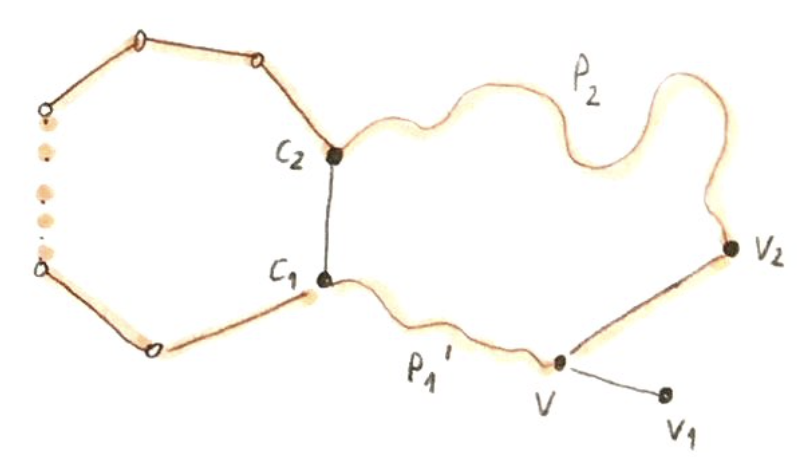
\includegraphics[width=80mm]{Slike/3_2.png}
            \caption{Primer, ko $v \in P_1$}\label{pot2}
        \end{figure}
        Ta cikel je res vsaj za 1 daljši, kar vidimo podobno kot v prejšnjem primeru.

\end{itemize}
V obeh primerih smo prišli v protislovje, torej $|C| \geq 2k$.
%%%%%%%%%%%%%%%%%%%%%%%%%%%%%%%%%%%%%%%%%%%%%%%%%%%%%%%%%%%%%%%%%%%%%%%%%%%%%%%%%%%%%%%%%%%%%%%%

\newpage
\section*{4. naloga}
Naj bo $k$ liho in $n$ sodo število, $n > k$. Naj bo $G$ graf, katerega vozlišča so elementi grupe $\mathbb{Z}_n$ in vozlišči $x, y$ povezani natanko tedaj, ko je $|x - y| \leq \frac{k - 1}{2}$ ali $x - y = \frac{n}{2}$. Določi povezanost grafa $G$.
\\
\\
$G$ je $k$-regularen za $k \geq 1$ in povezan za $k \geq 3$. Torej je povezanost grafa največ $k$, imamo torej pogoj $\kappa (G) \leq k$.
Opazimo, da za $k = n - 1$ dobimo polni graf $K_n$, ki ima povezanost $n - 1$. Zdi se, da bi povezanost lahko bila enaka $k$.
\\
Ker vemo, da $\kappa (G) \leq k$, moramo za dokaz $\kappa (G) = k$ pokazati še $\kappa (G) \geq k$, za kar uporabimo Mengerjev izrek.
\\
Naj bo $X$ poljubna podmnožica $V(G)$, da je $G - X$ nepovezan. Pokazati želimo, da mora biti $|X| \geq k$.
Po Mengerju v $G$ obstaja $k$ paroma neodvisnih poti med $u$ in $v$. Vemo, da morajo biti vsa vmesna vozlišča na teh poteh v $X$ (sicer bi bil G-X povezan).
Ker $u$ ni direktno povezan z $v$, mora biti $|X| \geq k$, torej je $\kappa(G) \geq k$.
\\
Ker velja $\kappa (G) \leq k$ in $\kappa (G) \geq k$ sledi, da je $\kappa (G) = k$.
%%%%%%%%%%%%%%%%%%%%%%%%%%%%%%%%%%%%%%%%%%%%%%%%%%%%%%%%%%%%%%%%%%%%%%%%%%%%%%%%%%%%%%%%%%%%%%%%

\newpage
\section*{5. naloga}
Dokaži ali ovrzi naslednje trditve.

\begin{enumerate}
    \item Vsak $k$-obarvljiv graf $G$ ima dobro $k$-barvanje, v katerem nek barvni razred vsebuje natanko $\alpha(G)$ vozlišč. \textit{Trditev ne drži.}
        \\
        Poiščimo protiprimer.
        Opazujmo graf na sliki.
        \begin{figure}[ht!]
            \centering
            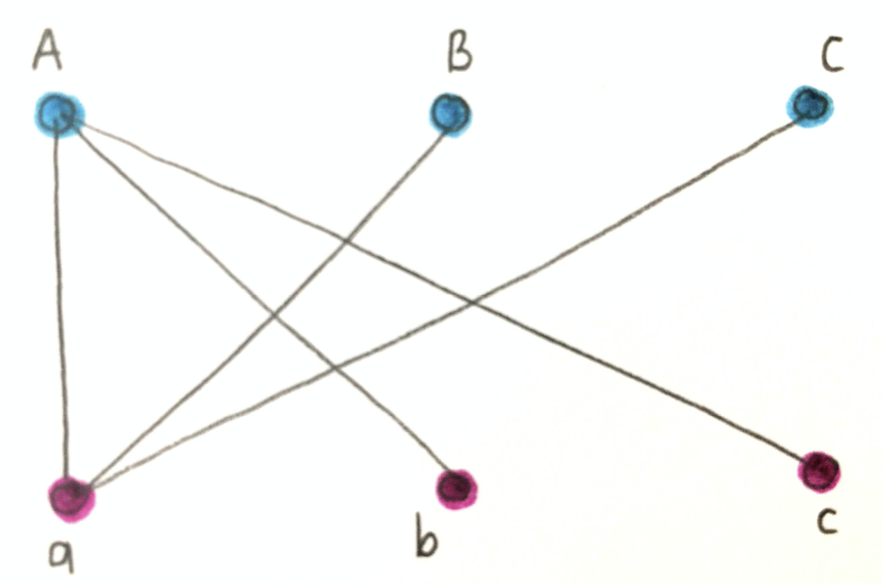
\includegraphics[width=80mm]{Slike/ABCabc.png}
            \caption{Graf za protiprimer.}
        \end{figure}

        \noindent
        Najprej opazimo, da moramo vozlišči $A$ in $a$ pobarvati vsako s svojo barvo, torej pristane v dveh različnih barvnih razredih.
        To nadalje pomeni, da sta $B$ in $C$ pobarvana z isto barvo kot $A$ ter $b$ in $c$ pobarvana z isto barvo kot $a$. 
        Celoten graf smo torej lahko pobarvali z dvema barvama, kar pomeni, da je graf $2$-obarvlljiv.
        Ker pa so v vsakem barvnem razredu po 3 vozlišča, je torej $\alpha(G) = 3$ in dobili smo protiprimer. Trditev res ne drži.


    \item Unija grafov $G$ in $H$ je graf z vozlišči $V(G) \cup V(H)$ in povezavami $E(G) \cup E(H)$. Velja $\chi(G \cup H) \leq \chi(G) + \chi(H)$. \textit{Trditev ne drži.}
        \\
        Poiščimo protiprimer.
        Vzemimo naslednja dva grafa $G$ in $H$
        \begin{figure}[ht!]
            \begin{minipage}{0.5\textwidth}
                \centering
                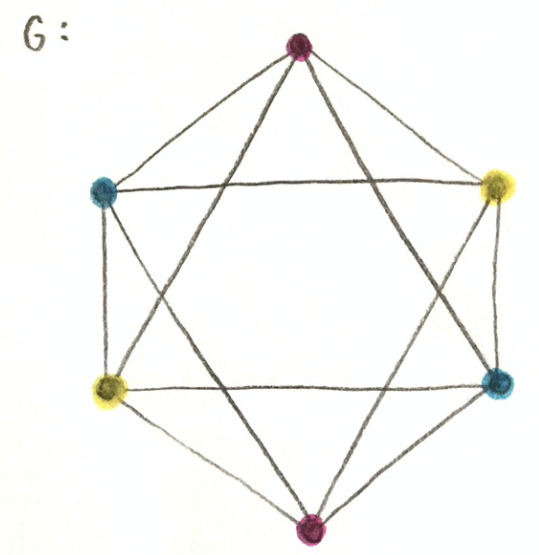
\includegraphics[width=50mm]{Slike/G.png}
                \caption{Graf $G$.}
            \end{minipage}\hfill
            \begin{minipage}{0.5\textwidth}
                \centering
                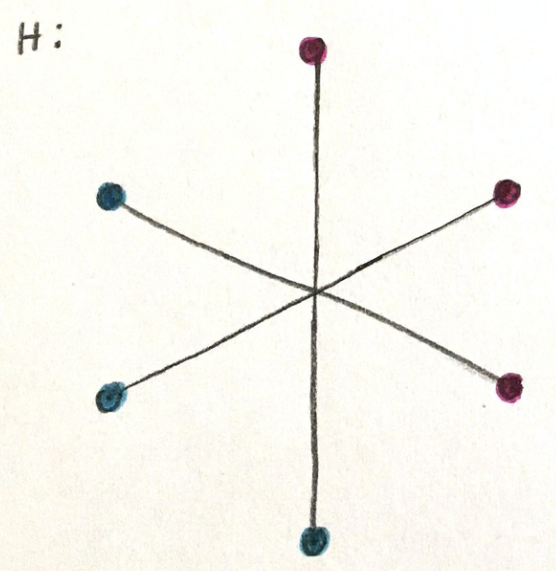
\includegraphics[width=50mm]{Slike/H.png}
                \caption{Graf $H$.}
            \end{minipage}\hfill
        \end{figure}

        \noindent
        Očitno je $\chi(G) = 3$ (2 ne more biti, ker vsebuje trikotnike) in $\chi(H) = 2$.
        Poglejmo sedaj še graf $G \cup H$.

        \begin{figure}[ht!]
            \centering
            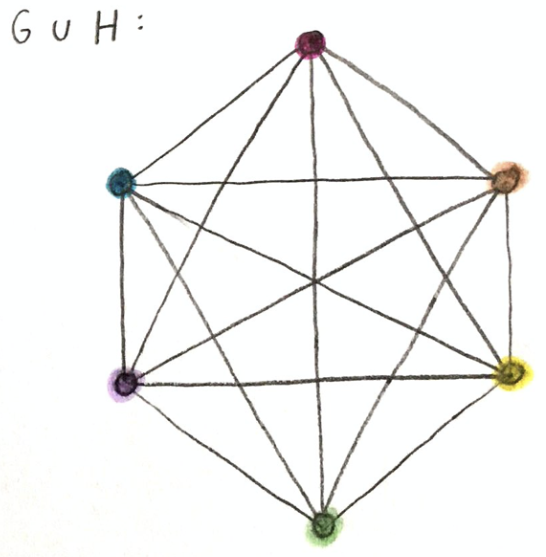
\includegraphics[width=60mm]{Slike/GinH.png}
            \caption{Graf $G \cup H$.}
        \end{figure}
        \noindent
        Graf $G \cup H$ je polni graf na $6$ vozliščih $K_6$, torej je $\chi(G \cup H) = 6$.
        \\
        Imamo $\chi(G \cup H) = 6$ in $\chi(G) + \chi(H) = 5$, torej smo našli protiprimer in enakost res ne drži.

    \item Če je $G$ graf, potem je $\chi(G) \leq n(g) - \alpha(G) + 1$. \textit{Trditev drži.}
        \\
        Naj bo $X$ neodvisna množica moči $\alpha(G)$. Vemo, da med vozlišči množice $X$ ni nobene povezave, torej lahko vsakemu vozlišču v množici $X$ lahko dodelimo isto barvo, ki jo označimo z $1$. 
        Sedaj pa pobarvajmo vsa ostala vozlišča v grafu, torej vseh $n(G) - \alpha(G)$ vozlišč, vsako s svojo barvo. Dobili smo dobro barvanje velikosti $n(G) - \alpha(G) + 1$. 
        To pomeni, da je kromatično število grafa $G$ največ $n(G) - \alpha(G) + 1$, torej res velja, da je $\chi \leq n(G) - \alpha(G) + 1$.
    
    \item Če je $G$ povezan graf, potem je $\chi(G) \leq 1 + a(G)$, kjer je $a(G)$ povprečna stopnja vozlišč grafa $G$. \textit{Trditev ne drži.}
        \\
        Poiščimo protiprimer.
        Imejmo graf $K_5$, ki mu iz nekega poljubnega vozlišča dodamo poljubno dolgo pot. Označimo tak graf z $G$.
        Če je pot dovolj dolga, se povprečna  stopnja vozlišč lahko zelo približa številu $2$ ($a(G) \simeq 2$). Kromatično število grafa $G$ je enako kromatičnemu številu $K_5$, kar je $5$.
        V tem primeru velja $\chi(G) > 1 + a(G)$, kar nam poda protislovje. Trditev torej ne drži.

\end{enumerate}


\end{document}


\begin{thebibliography}{99}

\end{thebibliography}